\documentclass{article}
\usepackage[utf8]{inputenc}
\usepackage{amsmath,amssymb}
\usepackage{paralist}
\usepackage{color}
\usepackage[detect-weight=true, binary-units=true]{siunitx}
\usepackage{pgfplots}
\usepackage{authblk}
\usepackage{url}
\usepackage{multirow}
\usepackage{booktabs}
\usepackage{hyperref}

\title{Machine Learning and Data Mining project:\\Leaf identification}
\author[1]{Michele Scomina}
\affil[1]{
    problem statement,
    solution design,
    solution development,
    data gathering,
    writing
}
\date{Course of AA $2023$-$2024$ - DIA - Ingegneria Elettronica e Informatica (IN20)}



\begin{document}

\maketitle



\section{Problem statement}
\subsection{Goal of the project}
The goal of this project is to identify the type of leaf based on a group of features, which are derived from both the shape and texture of the leaf.
The given solution must be able to classify the leaves in one of 30 categories of leaves.

\subsection{Formal definitions}
The problem can be formally defined as follows:
\begin{itemize}
    \item Let $X$ be the set of all possible leaves. Every element $x \in X$ is a leaf defined by a 14-dimensional attribute vector, representing various shape and texture features of the leaf.
    \item Let $Y$ be the set of all possible categories of leaves. Every element $y \in Y = \{0, 1, 2, ..., 29\}$ represents a unique category of leaves.
    \item Let $f: X \to Y$ be the function that assigns each leaf to its category based on its attributes.
    \item Let $D = \{(x^{(1)}, y^{(1)}), \ldots, (x^{(n)}, y^{(n)})\}$ be the dataset, where $x^{(i)} \in X$ and $y^{(i)} \in Y$.
    \item The goal is to learn a model $M$ from the dataset $D$ such that the argmax of $f'_{\text{predict}}: X \times M \to P_{Y}$\footnote{...where $P_{Y}$ is the set of all possible probability distributions over $Y$.} approximates $f$ as closely as possible, effectively classifying the leaves into their correct categories.
\end{itemize}


\section{Assessment and performance indexes}
Since classes are relatively balanced, but are expected to be composed of only a few samples, there's a risk of ill-defined metrics, 
as the model might not be able to predict some classes and might not have a properly defined precision, recall or F1-score for those classes.
Therefore, the weighted accuracy and the AUC (OvR) will be used as performance indexes. 
The confusion matrices and the multiclass ROC (OvR)$^{\cite{multiclass_roc}}$ will also be used to better assess the models' performances.


\section{Proposed solution}
\subsection{Data pre-processing}
In order to have any sort of meaningful evaluation of the models, the dataset $D$ has to be split into a training set $D_{\text{train}}$ and a test set $D_{\text{test}}$, 
in order to test the models for generalization on unseen data:

\begin{equation*}
    D_{\text{train}} = subbag(D, r) \quad \text{and} \quad D_{\text{test}} = D \setminus D_{\text{train}}
\end{equation*}

The split will be done with a $80$-$20\%$ ratio (r = 0.8) using a stratified shuffle, in order to avoid misrepresentation of classes:

\begin{equation*}
    \frac
        {|\{(x^{(i)}, y^{(i)}) \in D_{\text{train}} : y^{(i)} = c\}|}
        {|D_{\text{train}}|}
    \approx 
    \frac
        {|\{(x^{(i)}, y^{(i)}) \in D_{\text{test}} : y^{(i)} = c\}|}
        {|D_{\text{test}}|},
    \quad \forall c \in Y
\end{equation*}

\subsection{Types of models}
For this project, three different kinds of models will be trained, in order to determine which one performs best for the problem at hand:
\begin{itemize}
    \item \textbf{Random Forest}, $M = \{T_1, T_2,... T_k\}$ with each $T_i \in T_{(S_i \times \mathbb{R}) \cup P_{Y}}$, where $S_i \subset \{1,...,14\}$ is a random subset of 4 features.\footnote{The number of features was chosen based on the square root of the total number of dimensions ($\lceil\sqrt{14}\rceil = 4$).}
    \item \textbf{Soft Support Vector Classifier (OvR)}, $M = \{w, b\}$ such that $w \in \mathbb{R}^{14}$ and $b \in \mathbb{R}$.
    \item \textbf{Naive Bayes}, $M = \{P(Y), P(X|Y)\}$, with $P(Y)$ being the prior probabilities of the classes in $Y$, and $P(X|Y)$ being the likelihood of the features in $X$ given the classes in $Y$.
\end{itemize}
One thing to note is that, normally, multiclass SVCs do not output probabilities.
Therefore, the SVC will be used in conjunction with Platt scaling$^{\cite{platt1999probabilistic}\cite{wu2003probability}}$, in order to follow the formal definition of the problem of outputting probability distributions and calculate the multiclass ROC and AUC.


\subsection{Model training}
The hyperparameters will first be searched for each model using a grid search with a $k$-fold cross-validation on the training set\footnote{...if applicable.}:
\begin{equation*}
    P^{*} = 
    (p_{1}^{*}, p_{2}^{*}, \dots, p_{h}^{*}) = 
    \underset{p_{1}, p_{2}, \dots, p_{h}}{\text{argmax}}
        \left(\frac{1}{k}\sum_{i=1}^{k}\text{AUC}_{\text{OvR}}
            (M(p_{1}, p_{2}, \dots, p_{h}), 
            D_{\text{train}}^{(i)})
        \right)
\end{equation*}
The models will then be trained on the entire training set with the best hyperparameters found during the grid search:
\begin{equation*}
    M^{*} = f_{\text{learn}}{(D_{\text{train}}, P^{*})}
\end{equation*}



\section{Experimental evaluation}



\subsection{Data}
The dataset used for this project is the "leaf" dataset\footnote{https://archive.ics.uci.edu/dataset/288/leaf}, 
which comprises of 340 samples of simple leaves, evenly distributed among the 30 classes.



\subsection{Procedure}
The models will be searched for the best hyperparameters using a grid search, with a $5$-fold cross-validation on the training set.
They will then be trained with the found hyperparameters and evaluated using the performance indexes mentioned in the previous section, and the results will be compared to determine which model performs best for the problem at hand.
The chosen values for the hyperparameters are as follows:
\begin{itemize}
    \item \textbf{Random Forest}: 
    \begin{description}
        \item[$n_{\text{estimators}}$:] $\{10, 25, 50, 100, 200, 500, 1000\}$
        \item[$T_{\text{max\_depth}}$:] $\{1, 3, 5, 10, 15, 25, 50\}$
    \end{description}
    \item \textbf{Soft SVC}: 
    \begin{description}
        \item[$C$:] $\{0.1, 0.5, 1, 10, 100, 1000, 10000, 100000\}$
        \item[$K(x, x')$:] $\{\langle x, x' \rangle, (\gamma \langle x, x' \rangle)^3, \exp(-\gamma ||x-y||^2), \tanh(\gamma\langle x, x' \rangle)\}$\footnote{Respectively, the linear, polynomial, RBF and sigmoid kernels.}
        \item[$\gamma$:] $\{1, \frac{1}{n_{\text{features}}}, \frac{1}{n_{\text{features}} \cdot \text{Var}(X)}\}$
    \end{description}
\end{itemize}

\newpage


\subsection{Results and discussion}
The results of the grid search are as follows:

\begin{table}[h]
    \centering
    \begin{tabular}{c|c|c}
        \toprule
        Model & Hyperparameters & $T_{\text{search}}$ [ms] \\
        \midrule
        Random Forest & $n_{\text{estimators}} = 200, T_{\text{max\_depth}} = 10$ & 9879 \\
        Soft SVC & $C = 10000, K(x, x') = \textbf{RBF}, \gamma = \frac{1}{n_{\text{features}}}$ & 1615 \\
        \bottomrule
    \end{tabular}
    \caption{
        Best hyperparameters found during the grid search.
    }
    \label{tab:hyperparameters}
\end{table}

The models are then trained on the entire training set and evaluated on the test set, with the following results (averaged over 50 runs):

\begin{table}[h]
    \centering
    \begin{tabular}{c|c|c|c|c}
        \toprule
        Model & Weighted accuracy & $\text{AUC}_{\text{OvR}}$ & $T_{\text{train}}$ [ms] & $T_{\text{test}}$ [ms] \\
        \midrule
        Random Forest & 78.1\% & 0.9864 & 283.6 & 28.9 \\
        Soft SVC & 70.6\% & 0.9706 & 30.2 & 17.9 \\
        Naive Bayes & 74.4\% & 0.9791 & 1.2 & 15.3 \\
        \bottomrule
    \end{tabular}
    \caption{
        Results of the models on the test set.
    }
    \label{tab:results}
\end{table}

The confusion matrices and ROC curves of the models are as follows:

\begin{figure}[h]
    \centering
    \begin{minipage}{0.735\textwidth}
        \centering
        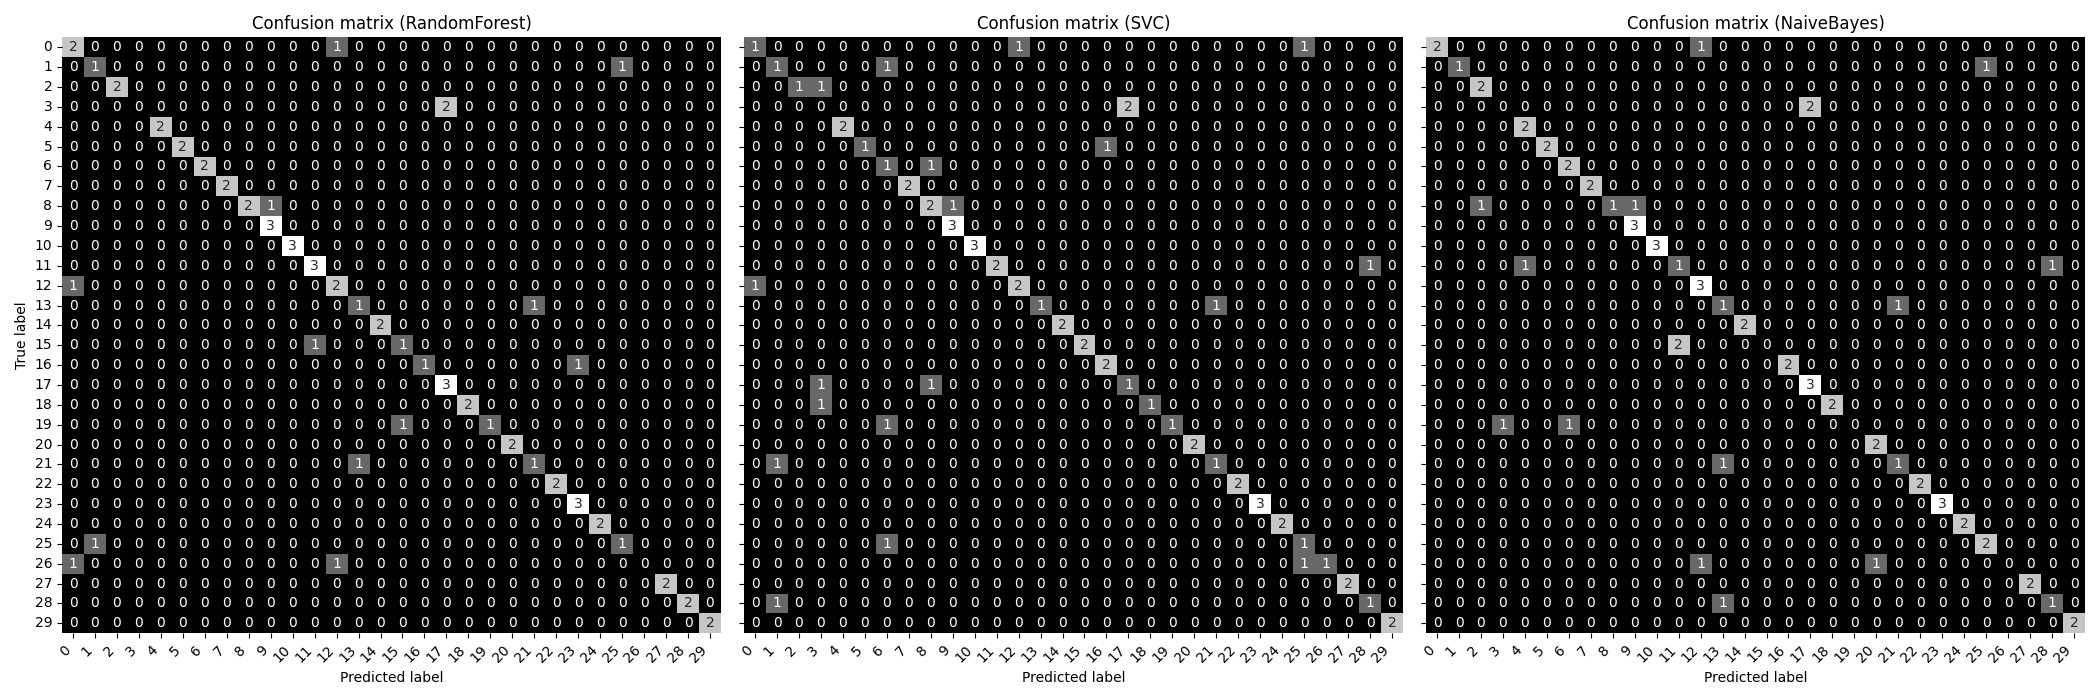
\includegraphics[width=\textwidth]{confusion_matrices.png}
        \label{fig:confusion_matrices}
    \end{minipage}\hfill
    \begin{minipage}{0.265\textwidth}
        \centering
        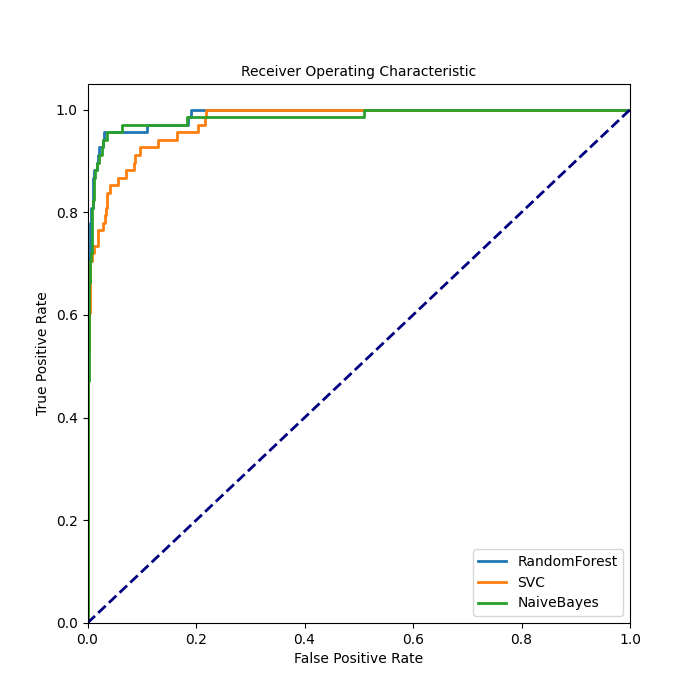
\includegraphics[width=\textwidth]{roc_curves.png}
        \label{fig:roc_curves}
    \end{minipage}
    \caption{
        Confusion matrices and ROC curves of the models.
    }
    \label{fig:results}
\end{figure}

The Random Forest model appears to be the best performing one for the "leaf" dataset, with the highest weighted accuracy and AUC,
at the cost of an expensive grid search and higher training and prediction times. It is, therefore, the recommended model when 
there isn't a strict constraint on the computational resources and when the highest performance is required.\\
The Naive Bayes model, with slightly lower performance indexes when compared to the Random Forest model,
but with a much lower training and prediction times and no need for grid search, is a good choice when
the computational resources are limited or when training time is a critical factor.\\
The Soft SVC model, instead, doesn't seem to perform as well as the other two models, with the lowest weighted accuracy and AUC,
and a relatively high training time compared to the Naive Bayes model. It is, therefore, the least recommended model for the "leaf" dataset.



\bibliographystyle{plain}
\bibliography{references}

\end{document}
